\setcounter{page}{2}

\section{Содержание задания}
Проект представляет собой создание карты города.
В проекте участвуют 16 разработчиков, бюджет проекта~---~50000 рублей, длительность проекта~---~6 месяцев.
Дата начала проекта~---~первый рабочий день марта текущего года.


\section{Внесение фактических данных}

Дата начала проекта в соответствии с базовым планом~---~03.03.2025, дата окончания проекта~---12.08.2025.
Затраты на проект в соответствии с базовым планом составляют 48945 рублей. 

По заданию дата отчета~---~11.05.2025.
Установка даты отчета показана на рисунке~\ref{fig:screen1}.

\begin{figure}[H]
	\centering
	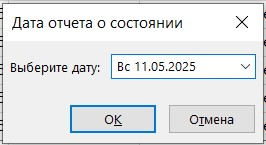
\includegraphics[width=0.9\textwidth]{img/screen1_report.jpg}
	\caption{Дата отчета}
	\label{fig:screen1}
\end{figure}

По заданию с 10 марта на 2 недели заболел 3D-аниматор.
В это время его обязанности выполнял художник-дизайнер, совмещая их со своими работами по проекту из расчета 60\% доступности по своим задачам и 40\% по задачам 3D-аниматора.
В этот период зарплата художника-дизайнера увеличилась на 10\%.

Необходимо установить 0\% занятости 3D-аниматора в период с 10.03 по 23.03 в связи с его болезнью, что продемонстрировано на рисунке~\ref{fig:screen2}. 

\begin{figure}[H]
	\centering
	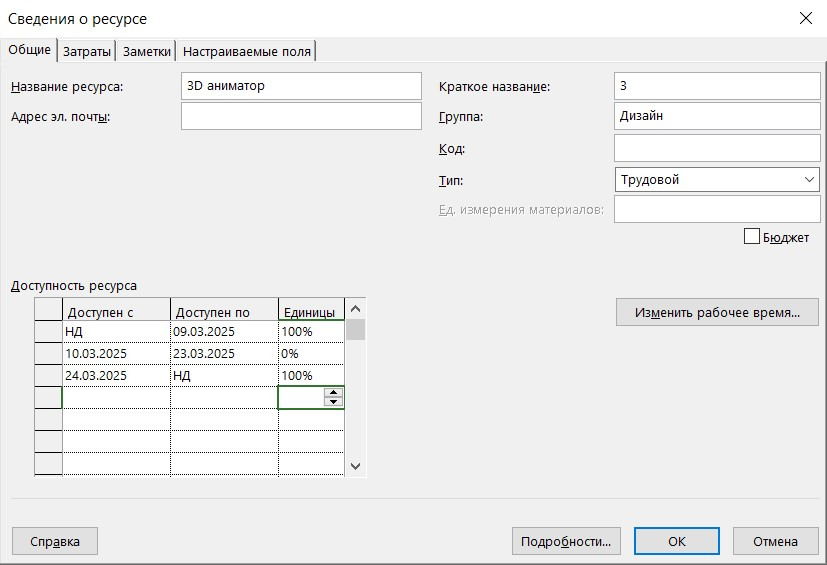
\includegraphics[width=0.9\textwidth]{img/screen2.jpg}
	\caption{Отражение информации о болезни 3D-аниматора}
	\label{fig:screen2}
\end{figure}

Также на этот период зарплата художника-дизайнера выросла на 10\%, обновленная стандартная ставка составила 8.8 рублей в час, а ставка сверхурочных~---13.2 рубля в час, что отражено на рисунке~\ref{fig:screen3}.
Занятость по собственным задачам у художника-аниматора составила 60\%, что отражено на рисунке~\ref{fig:screen4}.

\begin{figure}[H]
	\centering
	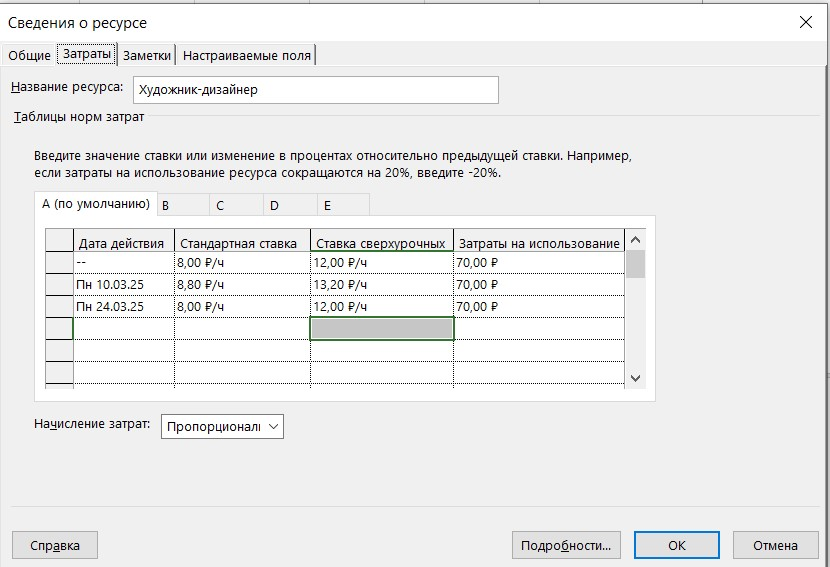
\includegraphics[width=0.9\textwidth]{img/screen3.jpg}
	\caption{Изменение ставки художника-дизайнера на период болезни 3D-аниматора}
	\label{fig:screen3}
\end{figure}

\begin{figure}[H]
	\centering
	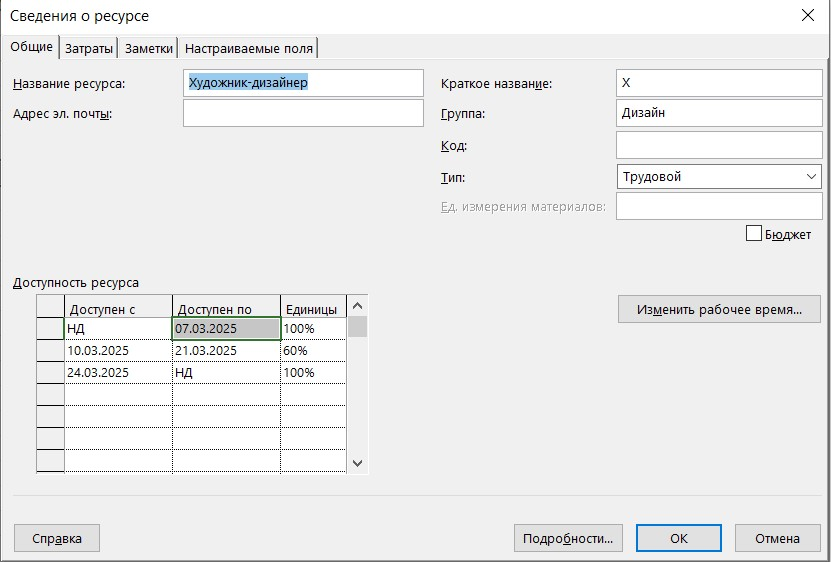
\includegraphics[width=0.9\textwidth]{img/screen4.jpg}
	\caption{Обновление нагрузки по собственным задачам художника-дизайнера}
	\label{fig:screen4}
\end{figure}

Задача <<Разработка 3D графических элементов>> 3D-аниматора, длящаяся с 03.03 по 17.03, попадает в период болезни 3D-аниматора, поэтому необходимо назначить на нее художника-дизайнера с 40\% занятости, что приведено на рисунке~\ref{fig:screen32}.

\begin{figure}[H]
	\centering
	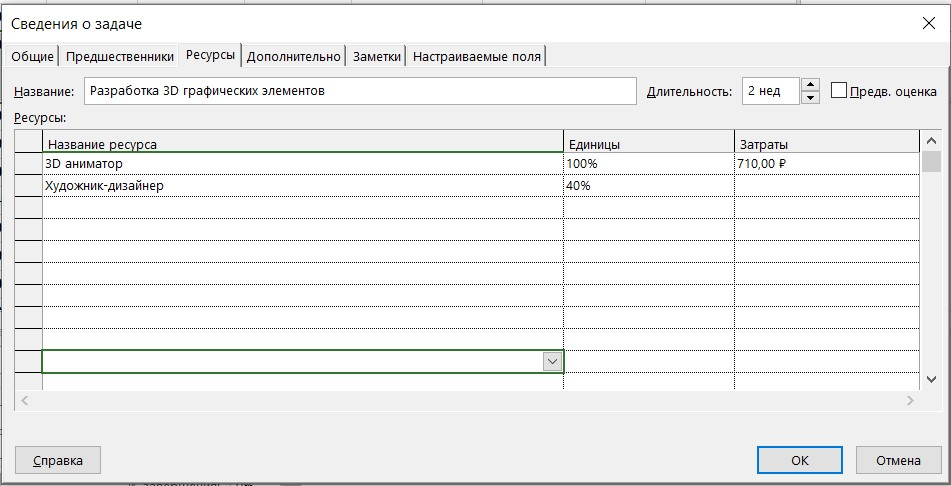
\includegraphics[width=0.9\textwidth]{img/screen32.jpg}
	\caption{Назначение художника-дизайнера на задачу 3D-аниматора}
	\label{fig:screen32}
\end{figure}

В представлении <<Использование задач>> необходимо указать сроки назначения художника-аналитика на задачу.
Из-за частичной загрузки художника-дизайнера дата окончания задачи <<Разработка 2D графических элементов>> смещается с 24.03 на 01.04, а дата окончания задачи <<Разработка 3D графических элементов>>~---~с 17.03 на 27.03.

Возникает перегрузка ресурса <<Художник-дизайнер>> из-за того, что на этот период его нагрузка ограничена 60\%, что составляет 4.8 часа в день, а задача <<Разработка 3D графических элементов>> вносит дополнительную нагрузку в 0.19 часа в день параллельно с задачей художника-аниматора <<Разработка 2D графических элементов>>.
Однако суммарная загрузка художника-аниматора за рабочий день не превышает 8 часов, что отражено на рисунке~\ref{fig:screen6}, поэтому данным предупреждением от Microsoft Project можно пренебречь.

\begin{figure}[H]
	\centering
	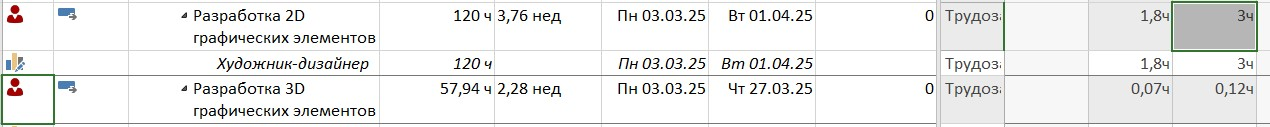
\includegraphics[width=0.9\textwidth]{img/screen6.jpg}
	\caption{Дневная загрузка художника-аниматора в период болезни 3D-дизайнера}
	\label{fig:screen6}
\end{figure}

Также на период болезни 3D-аниматора необходимо убрать его с совещаний.
Тем самым трудозатраты на совещания 12.03 и 19.03 сокращаются с 7 часов до 6 часов, что показано на рисунке~\ref{fig:screen7}.

\begin{figure}[H]
	\centering
	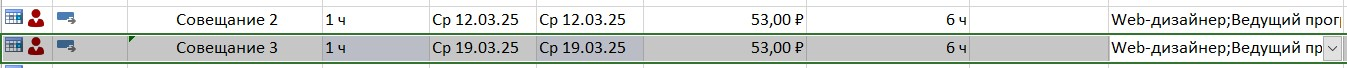
\includegraphics[width=0.9\textwidth]{img/screen7.jpg}
	\caption{Сокращение трудозатрат на совещания 12.03 и 19.03}
	\label{fig:screen7}
\end{figure}

Так как художник-дизайнер присутствует на совещании, необходимо указать для него занятость 100\% вместо установленных 60\% на этот период, что показано на рисунке~\ref{fig:screen8}.

\begin{figure}[H]
	\centering
	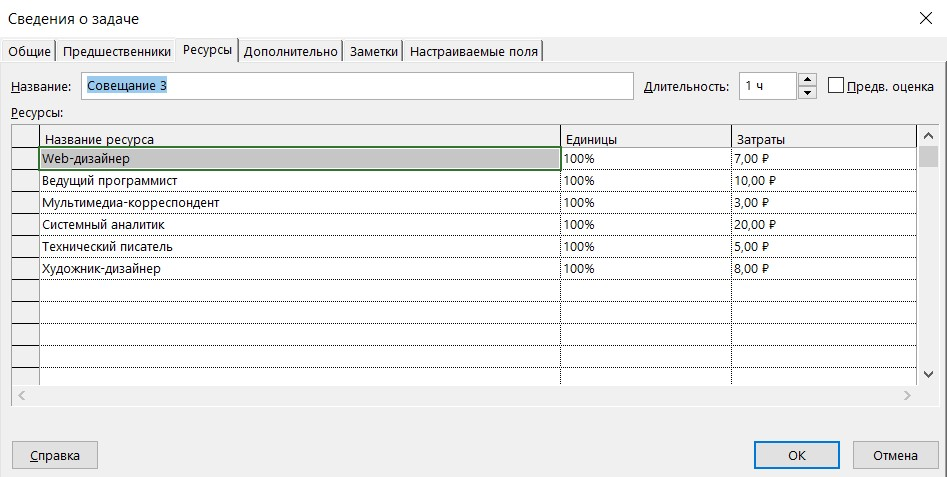
\includegraphics[width=0.9\textwidth]{img/screen8.jpg}
	\caption{Задание нагрузки художника-дизайнера на совещании}
	\label{fig:screen8}
\end{figure}

По заданию задача <<Разработка 3D графических элементов>> фактически завершилась 19.03, что необходимо отразить в разделе <<По графику>> --- <<Обновление задач>>, как показано на рисунке~\ref{fig:screen9}.

\begin{figure}[H]
	\centering
	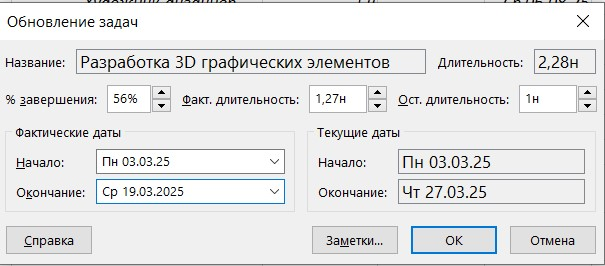
\includegraphics[width=0.9\textwidth]{img/screen9.jpg}
	\caption{Задание фактической даты окончания задачи <<Разработка 3D графических элементов>>}
	\label{fig:screen9}
\end{figure}

Обновленные даты занятости ресурсов для задачи <<Разработка 3D графических элементов>> приведены на рисунке~\ref{fig:screen10}.

\begin{figure}[H]
	\centering
	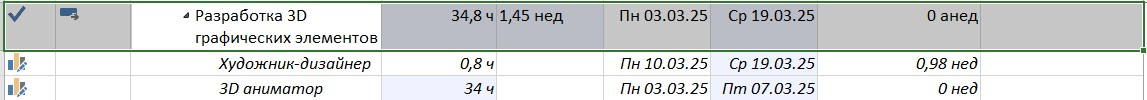
\includegraphics[width=0.9\textwidth]{img/screen10.jpg}
	\caption{Даты занятости ресурсов для задачи <<Разработка 3D графических элементов>>}
	\label{fig:screen10}
\end{figure}

Таким образом, дата начала задачи <<Создание заставки>> 3D-аниматора смещается на 24.03, однако так как по базовому плану она должна начинаться 17.03, на нее также необходимо назначить художника-дизайнера на 20.03 и 21.03, после чего с 24.03 ей будет заниматься выздоровевший 3D-аниматор.
Назначение художника-дизайнера на задачу <<Создание заставки>> приведено на рисунках~\ref{fig:screen33} и~\ref{fig:screen10_1}.

\begin{figure}[H]
	\centering
	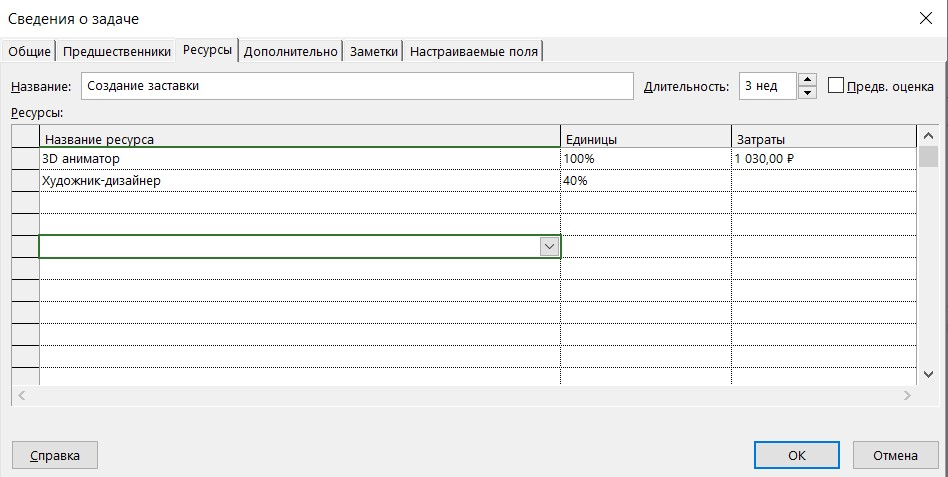
\includegraphics[width=0.9\textwidth]{img/screen33.jpg}
	\caption{Назначение художника-дизайнера на задачу <<Создание заставки>>}
	\label{fig:screen33}
\end{figure}

\begin{figure}[H]
	\centering
	
\includegraphics[width=0.9\textwidth]{img/screen10_1.jpg}
	\caption{Задание сроков занятости художника-дизайнера на задаче <<Создание заставки>>}
	\label{fig:screen10_1}
\end{figure}

Для художника-дизайнера возникают перегрузки, вызванные тем, что на этот период его нагрузка ограничена 60\%, что составляет 4.8 часа в день, а задача <<Создание заставки>> вносит дополнительную нагрузку в 3.01 часа в день, что суммарно не превосходит 8 часов в день, следовательно этой перегрузкой в Microsoft Project можно пренебречь.

\begin{figure}[H]
	\centering
	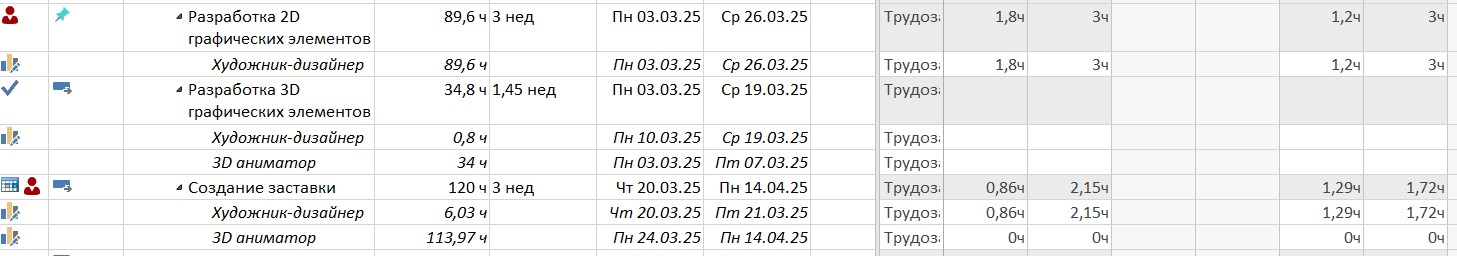
\includegraphics[width=0.9\textwidth]{img/screen16.jpg}
	\caption{Демонстрация занятости художника-дизайнера в период работы над задачей <<Создание заставки>>}
	\label{fig:screen16}
\end{figure}

По заданию с 01.04 совещания стали проводиться раз в две недели и на них должны присутствовать только ведущий программист, аналитик, мультимедиа-корреспондент, веб-дизайнер и технический писатель.

Ограничение старых совещаний показано на рисунке~\ref{fig:screen11}.

\begin{figure}[H]
	\centering
	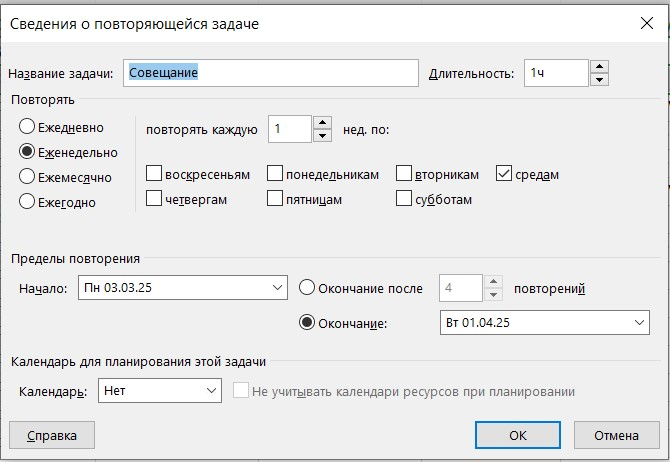
\includegraphics[width=0.9\textwidth]{img/screen11.jpg}
	\caption{Ограничение старых совещаний}
	\label{fig:screen11}
\end{figure}

Создание повторяющегося раз в две недели события новых совещаний, назначения им ресурсов и задания этим ресурсам ставки, не учитывающей затраты на использование, показаны на рисунках~\ref{fig:screen13}~---~\ref{fig:screen15}.

\begin{figure}[H]
	\centering
	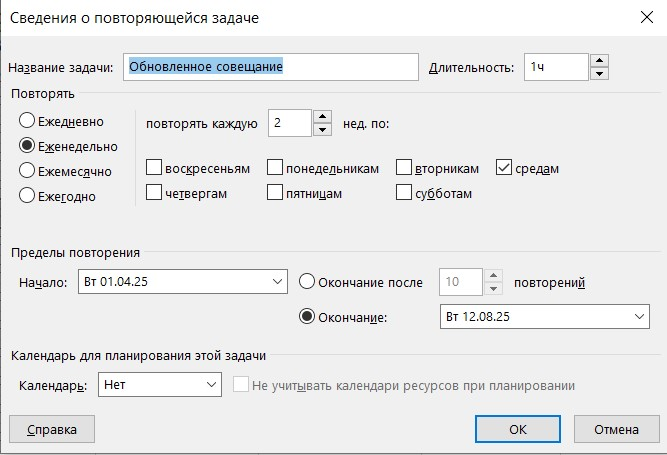
\includegraphics[width=0.9\textwidth]{img/screen13.jpg}
	\caption{Создание повторяющегося события новых совещаний}
	\label{fig:screen13}
\end{figure}

\begin{figure}[H]
	\centering
	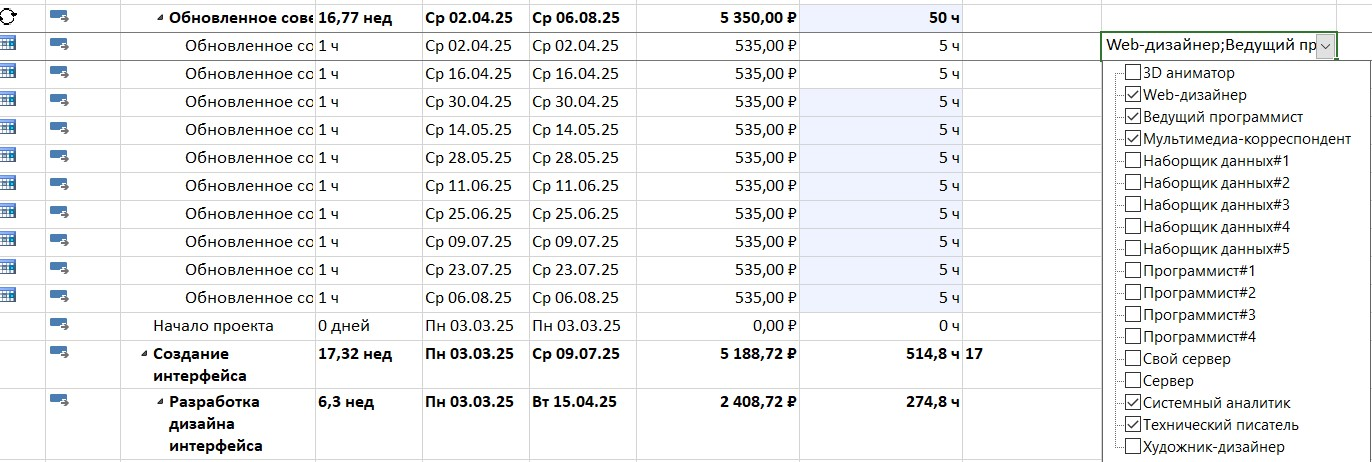
\includegraphics[width=0.9\textwidth]{img/screen14.jpg}
	\caption{Назначение ресурсов на новые совещания}
	\label{fig:screen14}
\end{figure}

\begin{figure}[H]
	\centering
	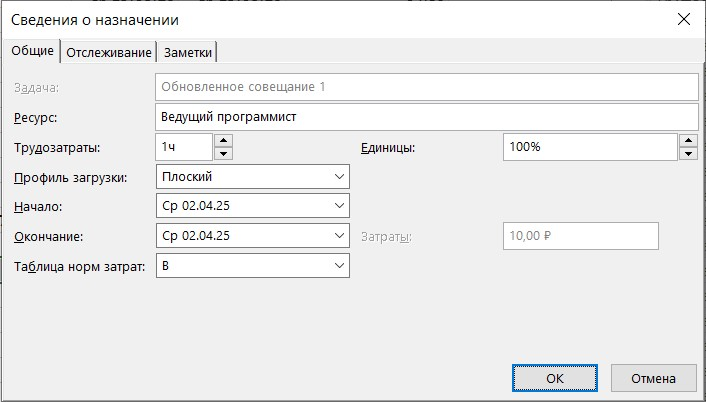
\includegraphics[width=0.9\textwidth]{img/screen15.jpg}
	\caption{Задание ставки без затрат на использование во время совещания}
	\label{fig:screen15}
\end{figure}

Полученные в итоге совещания приведены на рисунке~\ref{fig:screen12}.

\begin{figure}[H]
	\centering
	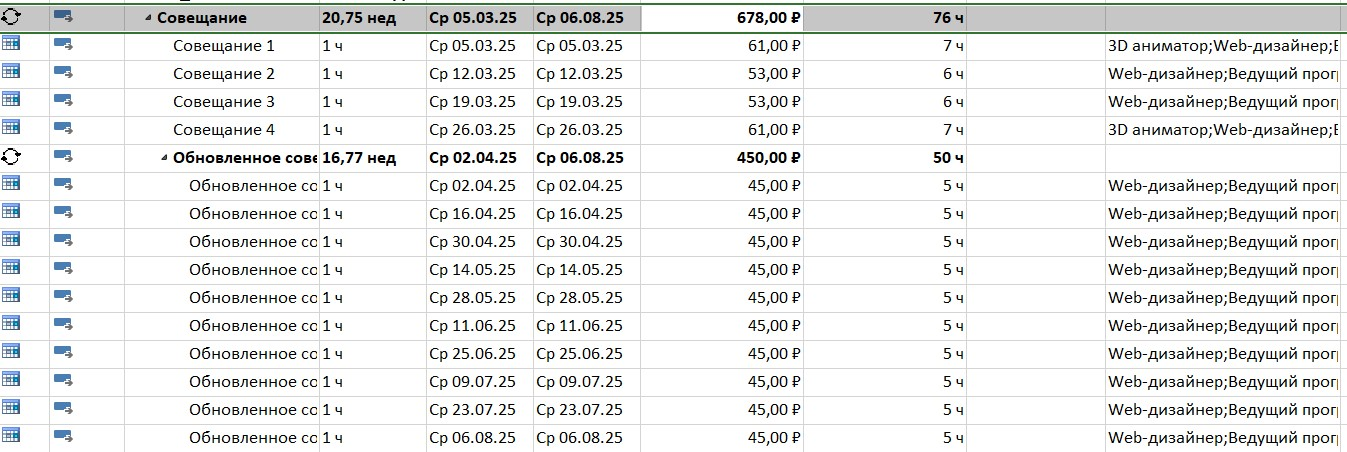
\includegraphics[width=0.9\textwidth]{img/screen12.jpg}
	\caption{Итоги по изменениям совещаний}
	\label{fig:screen12}
\end{figure}

Трудозатраты снизились с 159 часов до 76 часов, затраты~---~с 1387 рублей до 678 рублей, то есть трудозатраты и затраты на совещания удалось сократить более чем в 2 раза путем их проведения раз в 2 недели и участия в них более узкого круга специалистов с 1 апреля.

По заданию задачи <<Анализ и построение структуры базы объектов>> и <<Программирование средств обработки базы объектов>> фактически длились на 20\% дольше, то есть 2.4 и 3.6 недель вместо 2 и 3 недель соответственно.
Обновление фактической длительности задач представлено на рисунках~\ref{fig:screen17} и~\ref{fig:screen18}.

\begin{figure}[H]
	\centering
	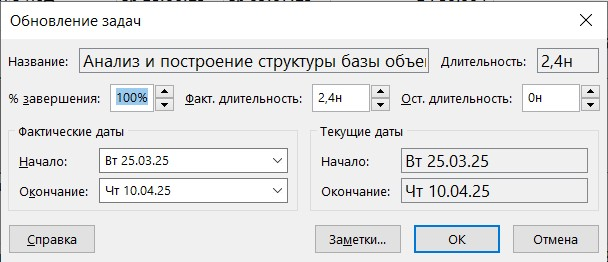
\includegraphics[width=0.9\textwidth]{img/screen17.jpg}
	\caption{Обновление фактической длительности задачи <<Анализ и построение структуры базы объектов>>}
	\label{fig:screen17}
\end{figure}

\begin{figure}[H]
	\centering
	
\includegraphics[width=0.9\textwidth]{img/screen18.jpg}
	\caption{Обновление фактической длительности задачи <<Программирование средств обработки базы объектов>>}
	\label{fig:screen18}
\end{figure}

При устранении перегрузок, возникших для программистов №3 и №4 в задаче <<Создание рабочей версии ядра>> из-за задержки по срокам задачи  <<Программирование средств обработки базы объектов>>, задача <<Создание рабочей версии ядра>> становится дольше на 1 день и завершается 19.06, что отражено на рисунках~\ref{fig:screen19} и~\ref{fig:screen20}.

\begin{figure}[H]
	\centering
	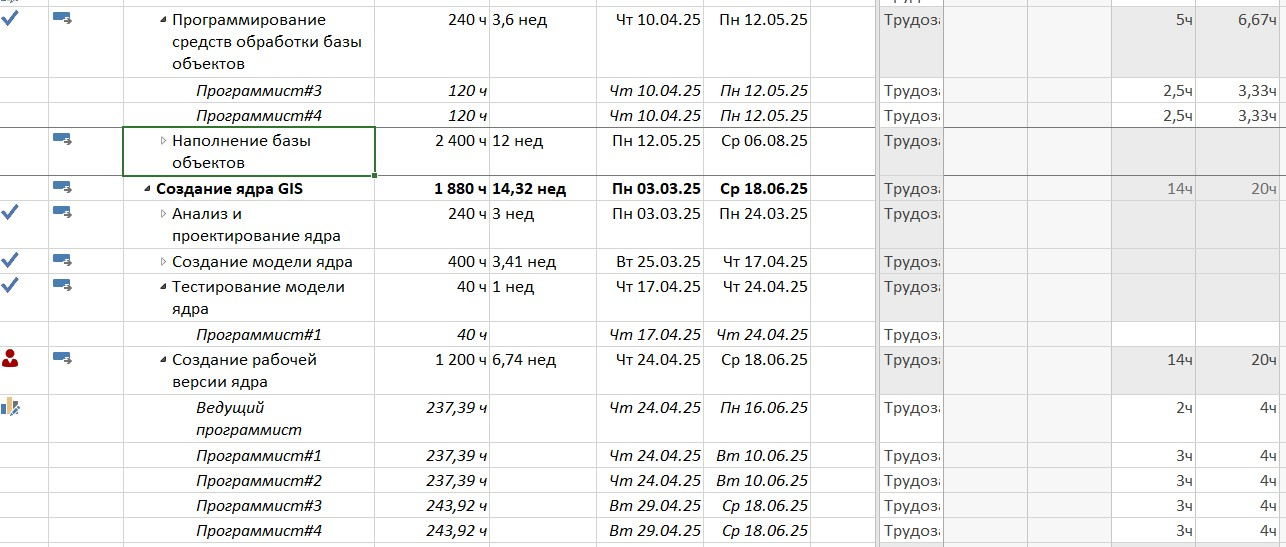
\includegraphics[width=0.9\textwidth]{img/screen19.jpg}
	\caption{Возникновение перегрузки в задаче <<Создание рабочей версии ядра>>}
	\label{fig:screen19}
\end{figure}

\begin{figure}[H]
	\centering
	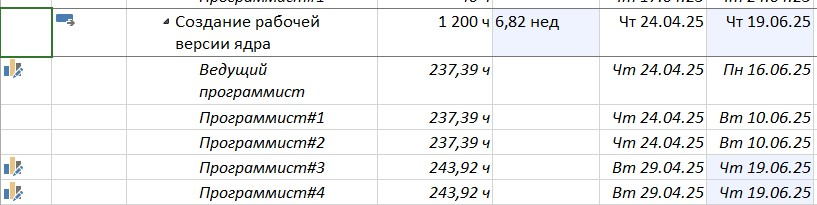
\includegraphics[width=0.9\textwidth]{img/screen20.jpg}
	\caption{Смещение даты окончания задачи <<Создание рабочей версии ядра>> после устранения перегрузок}
	\label{fig:screen20}
\end{figure}

Для остальных задач можно выставить, что они завершились вовремя, что достигается в разделе <<Проект>> --- <<Обновить задачу>>, как показано на рисунке~\ref{fig:screen34}.

\begin{figure}[H]
	\centering
	
\includegraphics[width=0.9\textwidth]{img/screen34.jpg}
	\caption{Фиксирование сроков завершения задач в отчетный период}
	\label{fig:screen34}
\end{figure}

По заданию с 01.04 было решено отказаться от аренды сервера, для чего был куплен собственный сервер за 4000 рублей.

Добавление нового сервера, являющегося материальным ресурсом, показано на рисунках~\ref{fig:screen21} и~\ref{fig:screen22}, отказ от аренды сервера~---~на рисунке~\ref{fig:screen23}.

\begin{figure}[H]
	\centering
	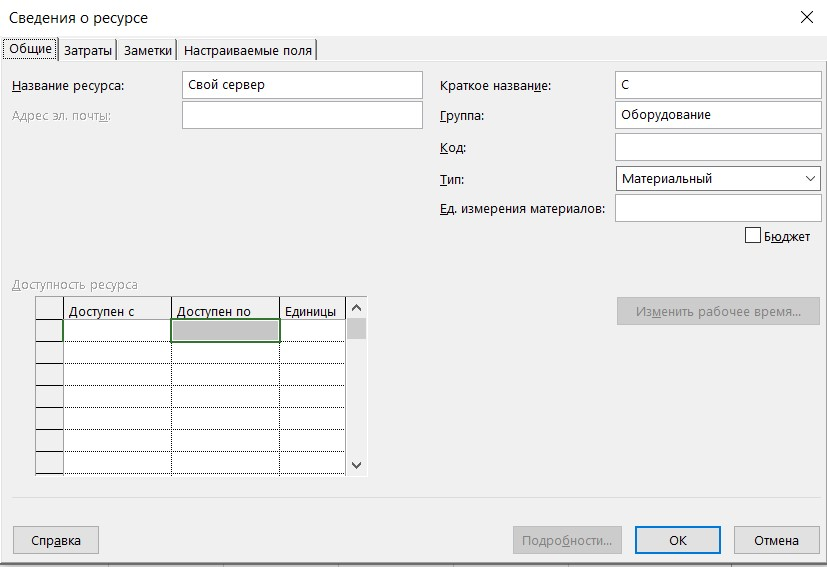
\includegraphics[width=0.9\textwidth]{img/screen21.jpg}
	\caption{Добавление нового сервера в качестве материального ресурса}
	\label{fig:screen21}
\end{figure}

\begin{figure}[H]
	\centering
	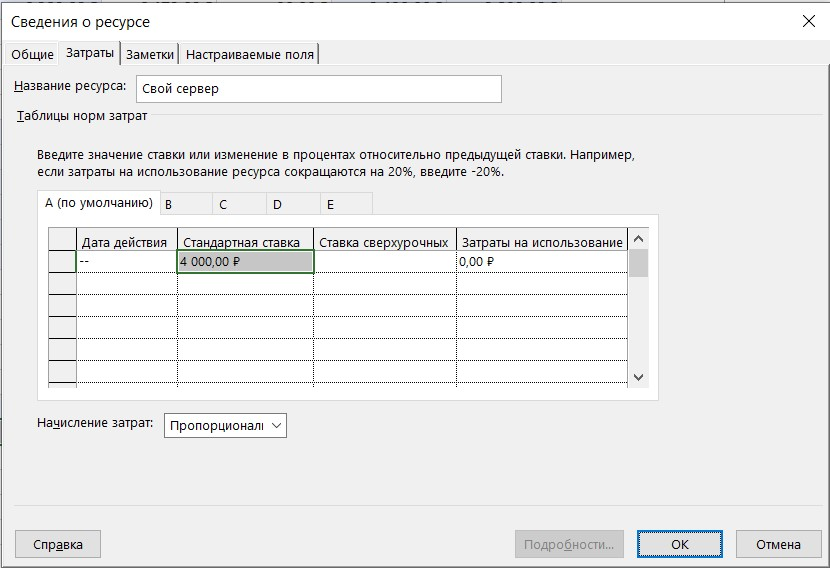
\includegraphics[width=0.9\textwidth]{img/screen22.jpg}
	\caption{Цена купленного сервера}
	\label{fig:screen22}
\end{figure}

\begin{figure}[H]
	\centering
	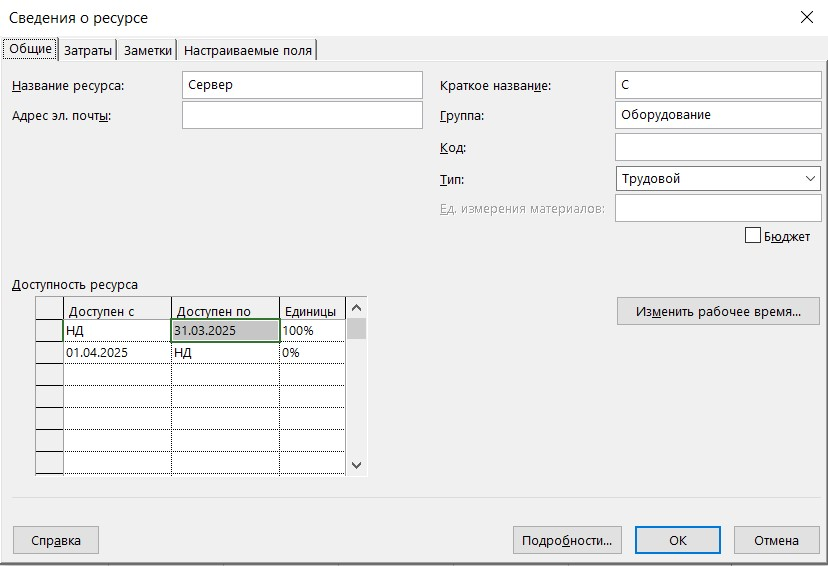
\includegraphics[width=0.9\textwidth]{img/screen23.jpg}
	\caption{Отмена аренды сервера}
	\label{fig:screen23}
\end{figure}

Необходимо добавить новый сервер в ресурсы вехи <<Построение базы объектов>>, а также указать дату окончания использования арендованного сервера (31 марта), что продемонстрировано на рисунках~\ref{fig:screen24} и~\ref{fig:screen25}.

\begin{figure}[H]
	\centering
	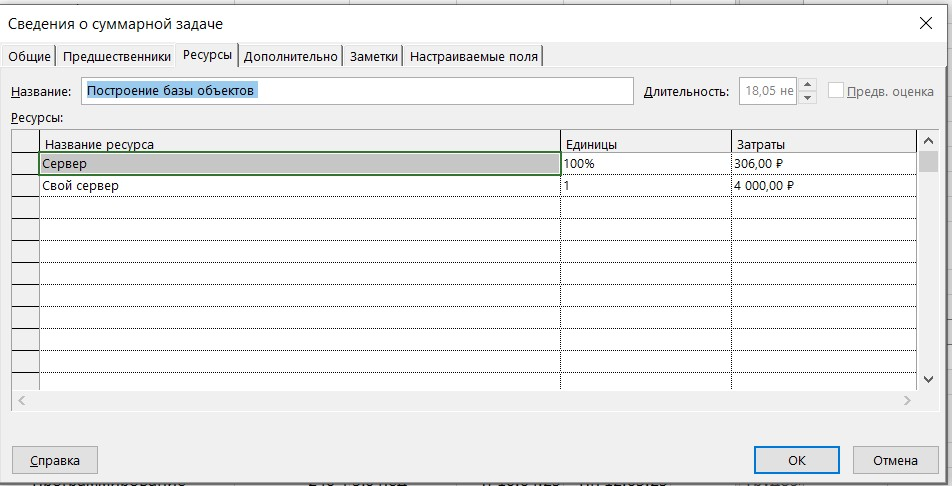
\includegraphics[width=0.9\textwidth]{img/screen24.jpg}
	\caption{Добавление нового сервера в вехе <<Построение базы объектов>>}
	\label{fig:screen24}
\end{figure}

\begin{figure}[H]
	\centering
	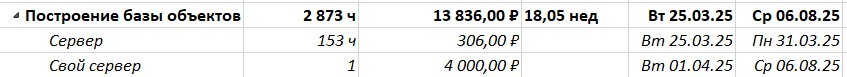
\includegraphics[width=0.9\textwidth]{img/screen25.jpg}
	\caption{Изменение сроков аренды сервера}
	\label{fig:screen25}
\end{figure}

Трудозатраты на использование арендованного сервера сократились с 3052 часов до 153 часов, затраты на аренду снизились с 6104 рублей до 306 рублей. 
Тем самым суммарные затраты на два сервера равны 4306 рублей, что почти в 1.5 раза меньше затрат на аренду сервера.

\section{Сравнение плановых и фактических показателей проекта}

Для сравнения плановых плановых и фактических показателей проекта были добавлены столбцы <<Базовое начало>>, <<Базовое окончание>>, <<Отклонение начала>>, <<Отклонение окончания>>, <<Базовые затраты>>, <<Отклонение по стоимости>>, <<Базовые трудозатраты>>, <<Отклонение по трудозатратам>>.
Резуьтаты приведены на рисунках~\ref{fig:screen26}~---~\ref{fig:screen28}.

\begin{figure}[H]
	\centering
	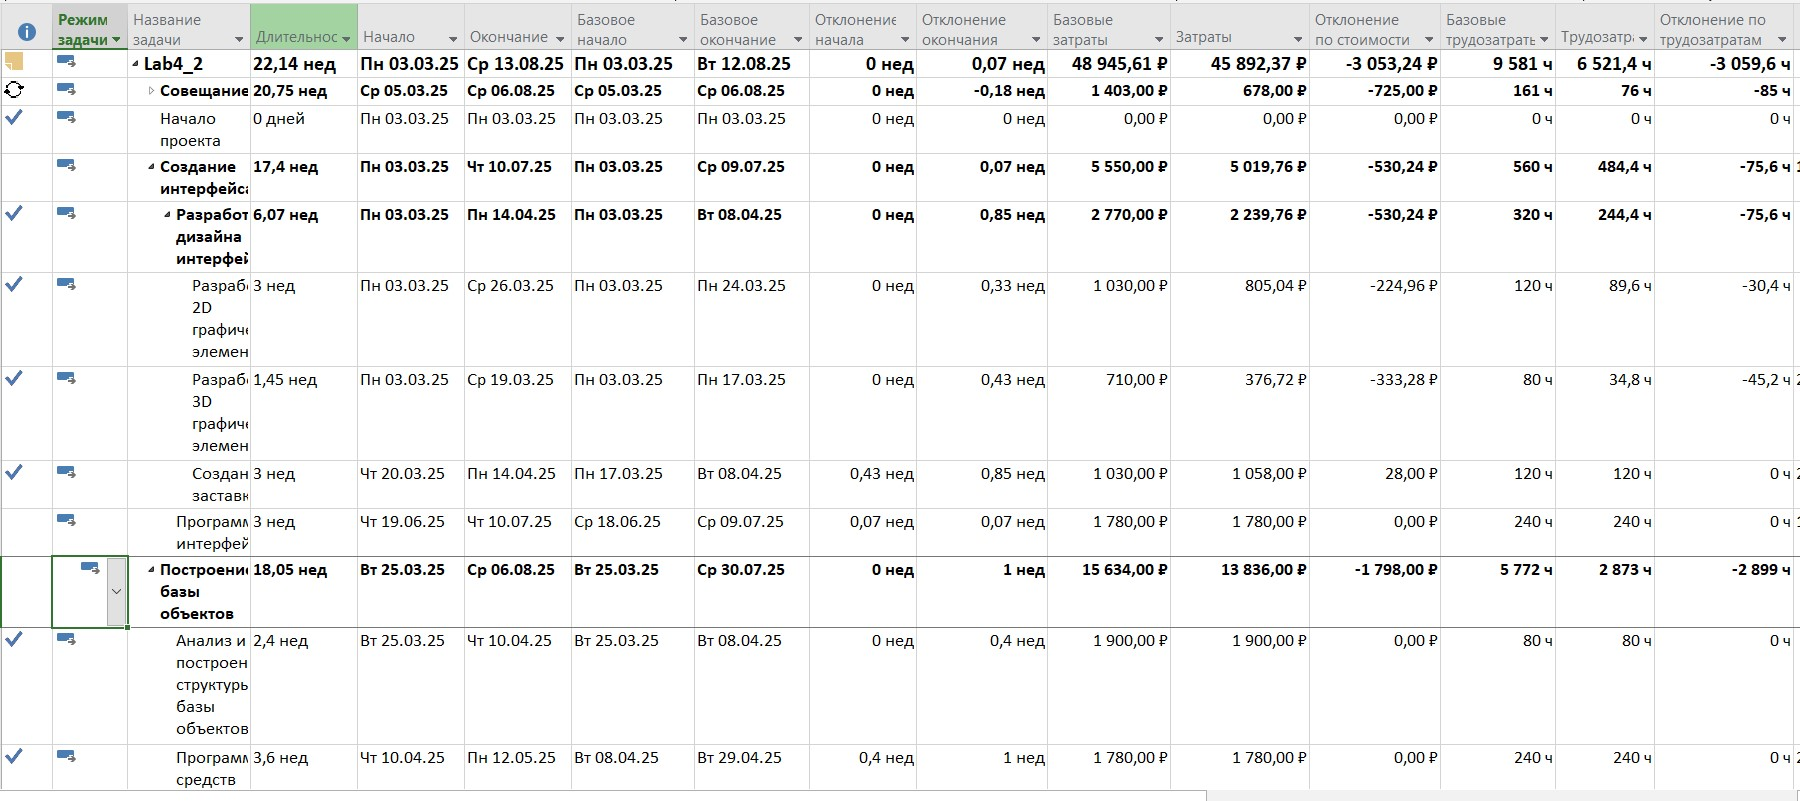
\includegraphics[width=0.9\textwidth]{img/screen26.jpg}
	\caption{Сравнение плановых и фактических показателей, часть 1}
	\label{fig:screen26}
\end{figure}

\begin{figure}[H]
	\centering
	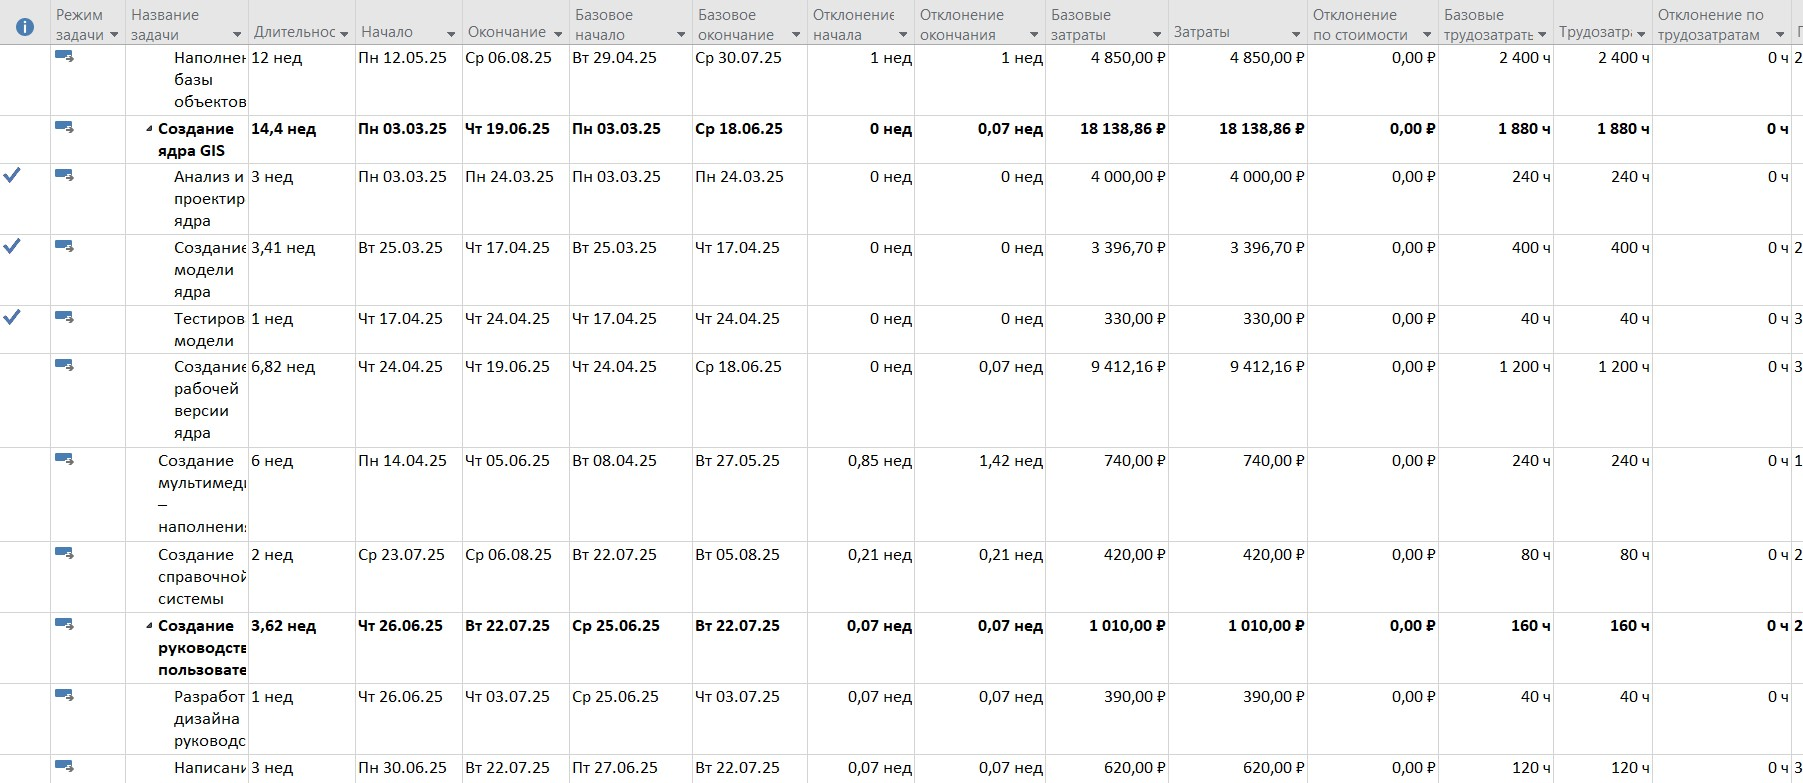
\includegraphics[width=0.9\textwidth]{img/screen27.jpg}
	\caption{Сравнение плановых и фактических показателей, часть 2}
	\label{fig:screen27}
\end{figure}

\begin{figure}[H]
	\centering
	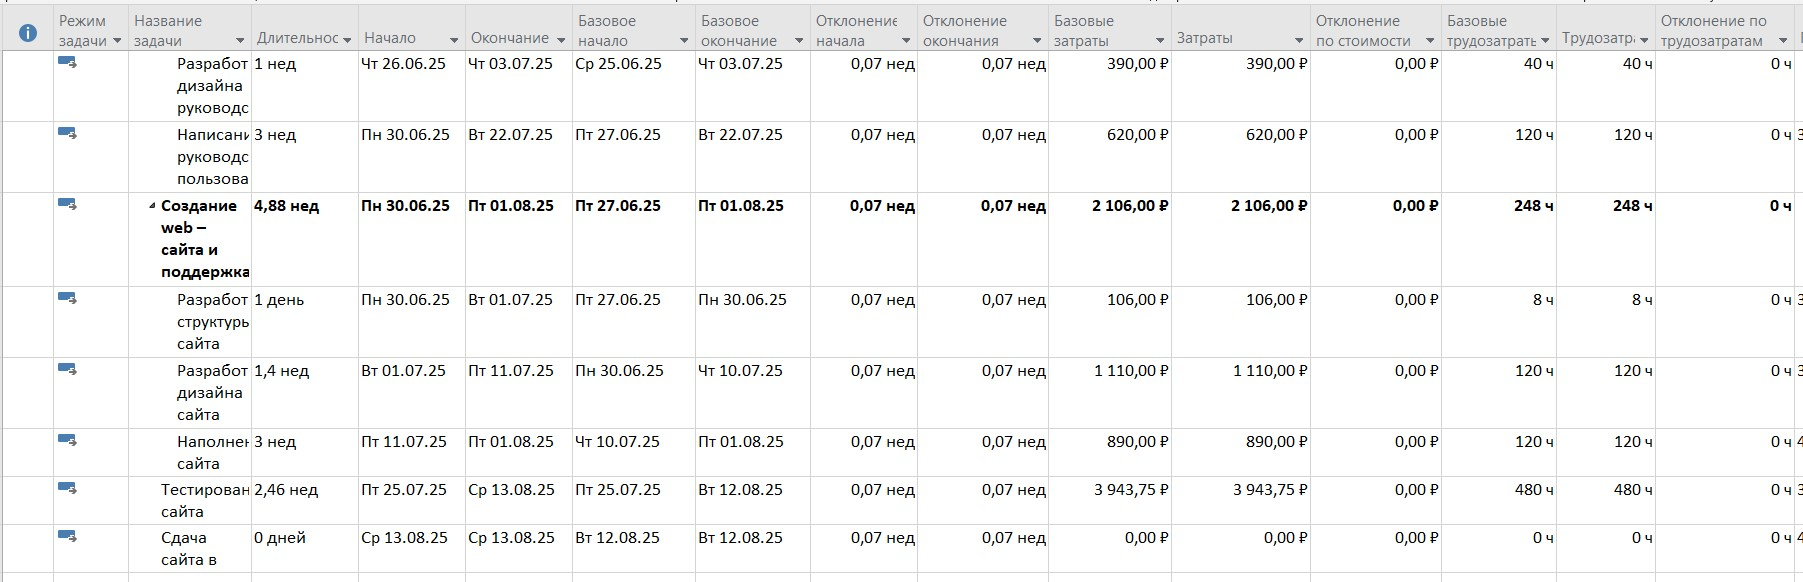
\includegraphics[width=0.9\textwidth]{img/screen28.jpg}
	\caption{Сравнение плановых и фактических показателей, часть 3}
	\label{fig:screen28}
\end{figure}

На рисунке~\ref{fig:screen35} приведена диаграмма Ганта с отслеживанием процентов завершения задач.

\begin{figure}[H]
	\centering
	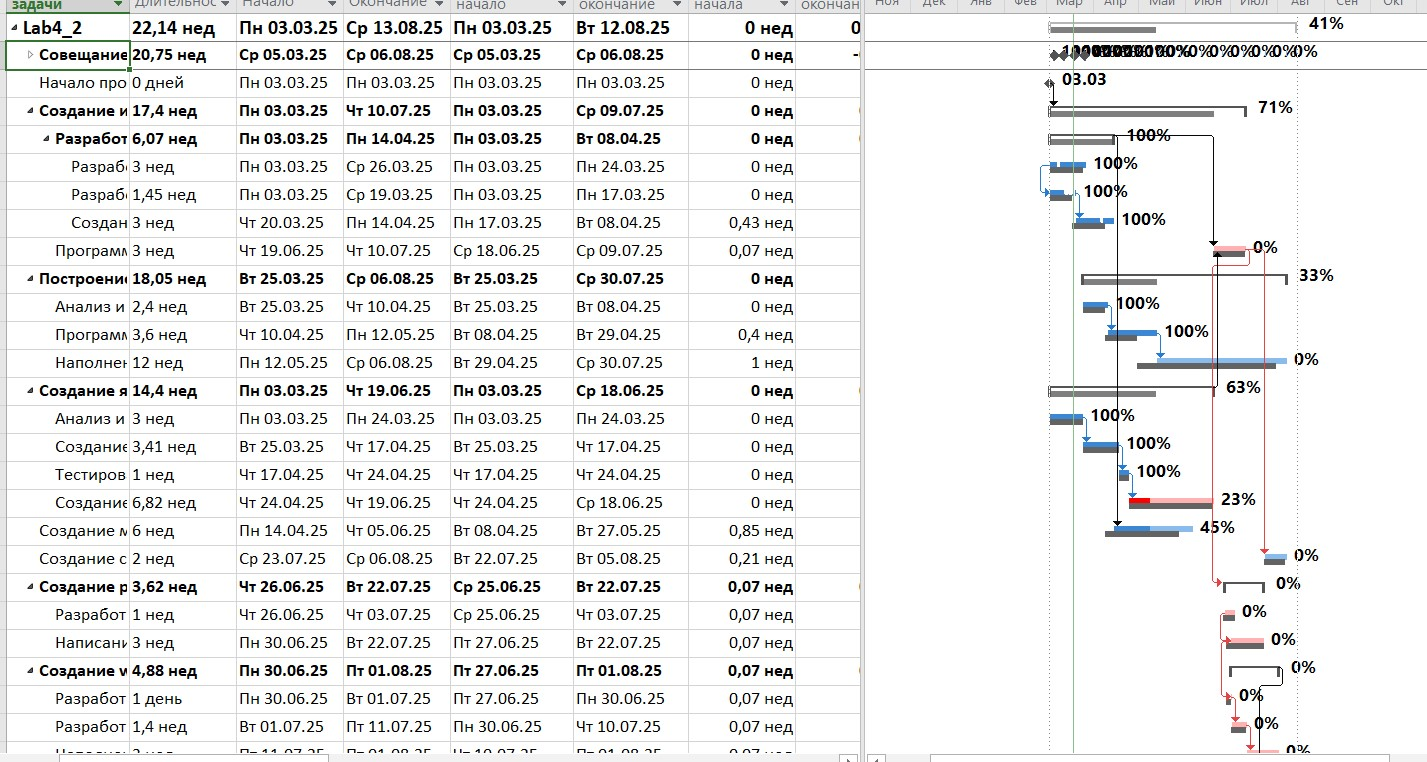
\includegraphics[width=0.9\textwidth]{img/screen35.jpg}
	\caption{Диаграмма Ганта с отслеживанием процентов завершения}
	\label{fig:screen35}
\end{figure}

На совещания потрачено меньше на 85 трудочасов, 725 рублей, чем было запланировано.

Создание интерфейса закончилось на день позже запланированного, что не является критичным.
На 11.05 (дата отчета) завершен 71\% работы в рамках этой вехи.
На него было потрачено на 530 рублей и 75 трудочасов меньше запланированного, основной вклад в это внесла веха разработки дизайна интерфейсов.
В ней на 224 и 333 рубля меньше, на 30.4 и 45.2 трудочаса меньше запланированного понадобилось на задачи разработки 2D и 3D графических элементов.
Также эта веха была завершена на 0.85 недели позже запланированного.

Веха <<Построение базы объектов>> заканчивается позже на неделю из-за задержки начала задачи <<Наполнение базы объектов>>.
На 11.05 завершено 33\%, что с учетом прогнозируемой задержки на неделю не является критичным, так как наборщики данных не задействованы больше ни в одной задаче.
На оценки отклонения трудозатрат и затрат для вехи может влиять неполная завершенность задач этой вехи.

Веха <<Создание ядра GIS>> задерживается на 0.07 недели, что не является критичным.
Завершение создания мультимедиа-наполнения на 1.42 недели позже не критично, так как от этой задачи ни одна другая не зависит.

Весь проект завершается 13.08, на день позже плана, что однако с запасом укладывается в сроки проекта.
По оценкам из отчета бюджет снизился на 3000 рублей.

\section{Линия прогресса}

Для отображения линии прогресса необходимо выполнить действия в разделе <<Формат>> --- <<Сетка>> --- <<Линии хода выполнения>>, показанные на рисунке~\ref{fig:screen29}.
Необходимо отобразить линию прогресса на дату отчета о состоянии проекта.

\begin{figure}[H]
	\centering
	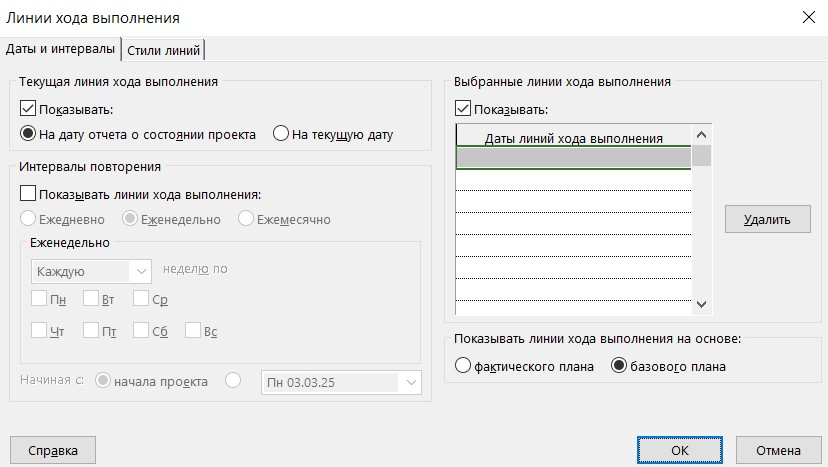
\includegraphics[width=0.9\textwidth]{img/screen29.jpg}
	\caption{Действия для отображения линии прогресса}
	\label{fig:screen29}
\end{figure}

Линия прогресса показана на рисунке~\ref{fig:screen30}.

\begin{figure}[H]
	\centering
	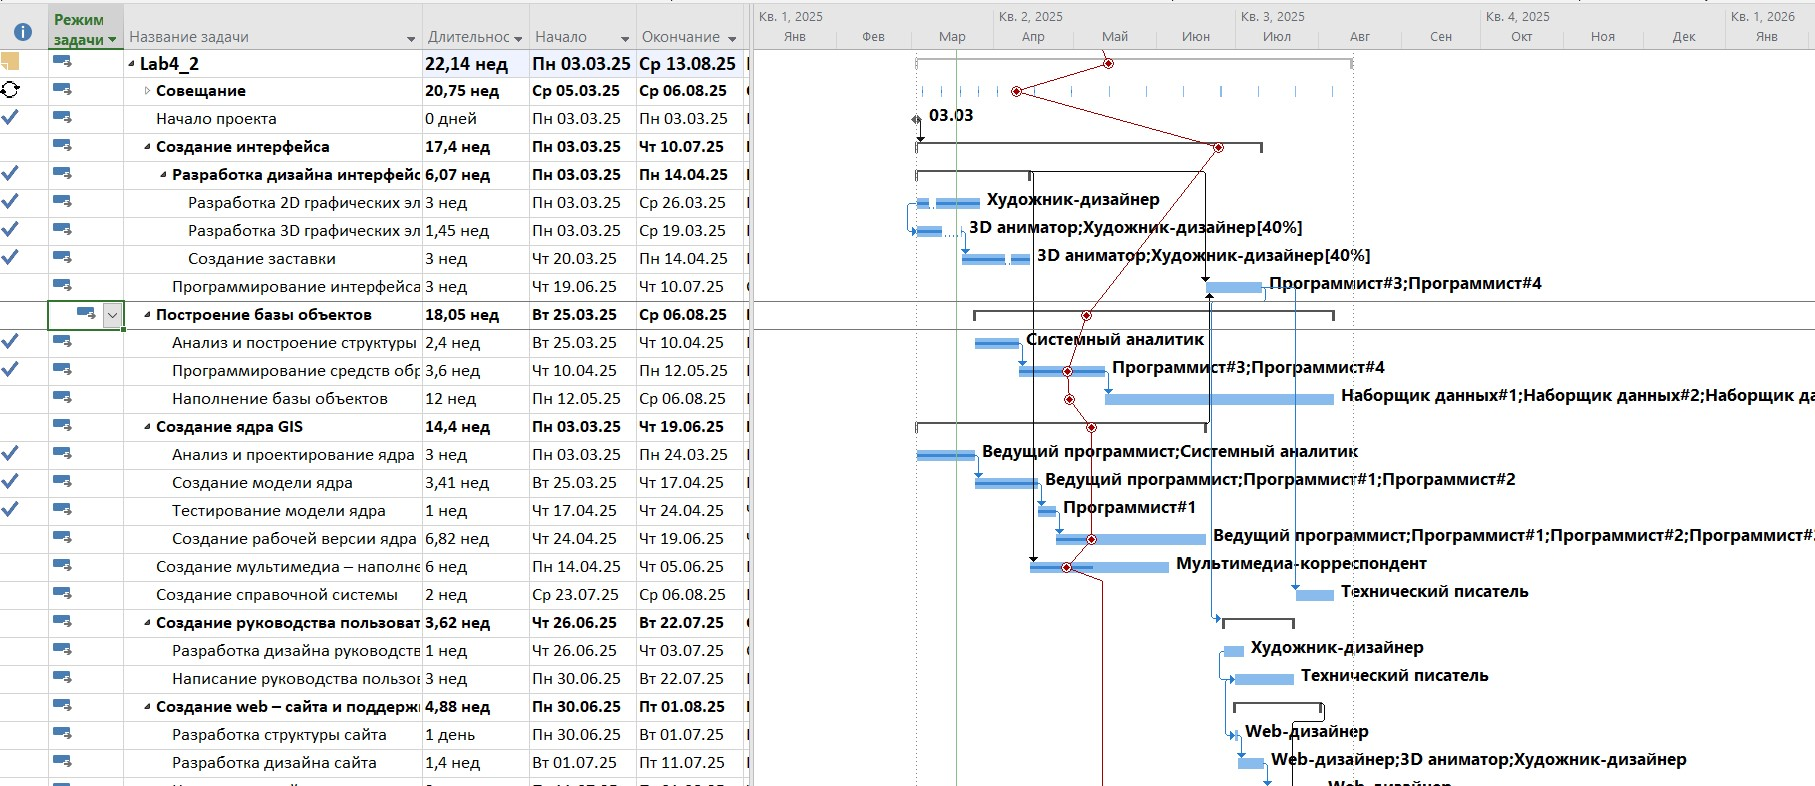
\includegraphics[width=0.9\textwidth]{img/screen30.jpg}
	\caption{Линия прогресса}
	\label{fig:screen30}
\end{figure}

По изгибу влево линии прогресса можно сказать, что веха <<Построение базы объектов>> отстает по срокам от заданных в базовом плане дат.
Самое большое отставание заметно у задачи <<Наполнение базы объектов>>, однако, как описывалось ранее, оно не является критичным.

\section*{Вывод}

Исходя из проведенного анализа на основе базового отчета было выявлено, что отклонение окончания составляет 0.07 недели, что не является критическим, так как проект укладывается в сроки, завершаясь 13.08.
Исходя из анализа отклонения затрат следует, что потрачено на 3053 рубля меньше запланированного. 
Затраты составляют 45892, что увеличивает запас бюджета, однако все еще может быть критичным.
